\documentclass[11pt]{article}

\usepackage{fullpage}
\usepackage{graphicx}
\usepackage{amsmath}
\usepackage{amssymb}
\usepackage{amsthm}
\usepackage{fancyvrb}
\usepackage{fancyhdr}
\usepackage{mdframed} % for problem and answer environments

% useful package
\usepackage[obeyspaces]{url}
\usepackage{listings}  % coding blocks
\usepackage[svgnames]{xcolor}
\graphicspath{ {./pic/} }

% codign block setting
\definecolor{codegreen}{rgb}{0,0.6,0}
\definecolor{codegray}{rgb}{0.5,0.5,0.5}
\definecolor{codepurple}{rgb}{0.58,0,0.82}
\definecolor{backcolour}{rgb}{0.95,0.95,0.92}

\lstdefinestyle{mystyle}{
    backgroundcolor = \color{backcolour},   
    commentstyle = \color{codegray},
    keywordstyle = \color{blue},
    numberstyle = \tiny\color{codegray},
    stringstyle = \color{codegreen},
    basicstyle = \ttfamily\footnotesize,
    breakatwhitespace=false,         
    breaklines=true,    captionpos=b,                    
    keepspaces=true, numbers=left,
    numbersep=2pt, showspaces=false,                
    showstringspaces = true, showtabs = true, tabsize = 2}
\lstset{style=mystyle}

\newenvironment{solution}{%
  \renewcommand\qedsymbol{$\blacksquare$}%
  \begin{mdframed}[backgroundcolor=gray!15]%
  \begin{proof}[Solution]}%
  {\end{proof}%
  \end{mdframed}}%



\parindent0in
\pagestyle{plain}
\thispagestyle{plain}


%% UPDATE MACRO DEFINITIONS %%
\newcommand{\myname}{Xiang Jyun, Jhang}
\newcommand{\assignment}{Homework 3}
\newcommand{\duedate}{March 31, 2024}

%% mathematical notation
\newcommand{\ept}{\mathbb{E}}
\newcommand{\pr}{\mathbb{P}}
\newcommand{\normal}{\mathcal{N}}
\newcommand{\var}{\text{Var}}
\newcommand{\cov}{\text{Cov}}
\newcommand{\given}{\,|\,}
\newcommand{\defas}{\overset{\Delta}{=}}


\begin{document}


\textbf{National Taiwan University}\hfill\textbf{\myname}\\[0.01in]
\textbf{ECON 5211 Labor Economics I}\hfill\textbf{\assignment}\\[0.01in]
\textbf{Prof.\ Kuan Ming, Chen}\hfill\textbf{\duedate}\\
\smallskip\hrule\bigskip


% question 1
\section{Normalization of the Selection Equation}

    In class, we said that 
    \[
        \text{ATT} = \int_{0}^{1} \text{MTE}(u) \frac{\pr(p(Z)\geq u)}{\pr(D=1)}du 
    \] 
    This result relies on the following normalization.
    \[ 
        D = 1\{U \leq v(Z)\} = 1\{\tilde{U} \leq p(Z)\} 
    \]
    where $p$ is the propensity score.
    \begin{enumerate}

        % Q1-1
        \item We write $D = 1\{F_U(U) \leq F_U(v(Z))\}$, where \( F_U \) is the CDF of the continuously distributed \( U \). What is the distribution of \( F_U(U) \)? Let \( \tilde{U} := F_U(U) \) from now on.
        
            \begin{solution}
                Given $U$ is a continuously distributed random variable, its CDF is also a continuous distribution. From the Statistics lecture we learned that, the CDF of any random variable follows uniform $[0,1]$, so $\tilde{U} \sim \text{Uniform}[0,1]$.
            \end{solution}
        
        % Q1-2
        \item Define \( p(z) := P(D = 1|Z = z) \), show that \( p(z) = F_U(v(z)) \).
        
            \begin{solution}
                Given the definition of $p(z)$, we can obtain
                \[ \begin{aligned}
                    p(z) &\defas \pr(D=1 \given Z=z) && \\
                         &= \pr(F_U(U) \leq F_U(v(z))) && \text{(Definition)} \\
                         &= F_U(v(z)) && (F_U(U) \sim \text{Uniform}[0,1])
                \end{aligned} \]
            \end{solution}
        
        % Q1-3
        \item Show that $D = 1\{\tilde{U} \leq p(Z)\}$.
        
            \begin{solution}
                Starting from the definition of $D$ in (a), note that $\tilde{U} \defas F_U(U)$ and the result in (b) shows that $p(z) = F_U(v(z))$, so
                \[ \begin{aligned}
                    D &= 1\{F_U(U) \leq F_U(v(z))\}  \\
                      &= 1\{\tilde{U} \leq p(z)\} 
                \end{aligned} \]
            \end{solution}
        
    \end{enumerate}


% question 2
\section{Derivation of the Weights for LATE}

    In this exercise, we try to show that LATE of instrument \( z \) and \( z' \) can be written as:
    \[ \text{LATE}_{z'}^{z} = \frac{E[Y|Z=z] - E[Y|Z=z']}{E[D|Z=z] - E[D|Z=z']} = \int_{0}^{1} \text{MTE}(u) \times \frac{1\{u \in [p(z'),p(z)]\}}{p(z) - p(z')} du \]

    \begin{enumerate}

        % Q2-1
        \item Which part of the most right-hand side is \( E[D|Z=z] - E[D|Z=z'] \) corresponding to?
        
            \begin{solution}
                The denominator $p(z) - p(z')$, which represents the change of potential treatment status.
            \end{solution}

        % Q2-2
        \item Show that \( E[Y|Z=z] = E[Y_1|U \leq p(z)]p(z) + E[Y_0|U > p(z)](1 - p(z)) \)
        
            \begin{solution}
                Note that we implicitly assume $U \sim \text{Uniform}[0,1]$, so we can derive the following result from definition:
                \[ \begin{aligned}
                    &\ept(Y \given Z=z) \\
                    =\ & \ept(Y \given D=1, Z=z) \cdot \pr(D=1 \given Z=z) + \ept(Y \given D=0, Z=z) \cdot \pr(D=0 \given Z=z) \\
                    =\ & \ept(Y \given D=1, Z=z) \cdot \pr(U \leq p(z) \given Z=z) + \ept(Y \given D=0, Z=z) \cdot \pr(U \geq p(z) \given Z=z) \\
                    =\ & \ept(Y_1 \given U \leq p(z)) \cdot p(z) + \ept(Y_0 \given U \geq p(z)) \cdot (1-p(z))
                \end{aligned} \]
            \end{solution}
        
        % Q2-3
        \item Show that \( E[Y|Z=z] = \int_{0}^{p(z)} E[Y_1|U = u] du + \int_{p(z)}^{1} E[Y_0|U = u] du \)
        
            \begin{solution}
                Given the preceding result, we further derive that:
                \[ \begin{aligned}
                    &\ept(Y_1 \given U \leq p(z)) \cdot p(z) + \ept(Y_0 \given U \geq p(z)) \cdot (1-p(z))  \\
                    =\ & \int_{0}^{p(z)} \ept[Y_1 \given U =u] \,\text{d}u + \int_{p(z)}^{1} \ept[Y_0 \given U =u] \,\text{d}u 
                \end{aligned} \]
                where the former term capture the average $Y_1$ for those with $u \in [0, p(z)]$; while the latter term capture the average $Y_0$ for those with $u \in [p(z), 1]$
            \end{solution}
        
        % Q2-4
        \item Show that \( E[Y|Z=z] - E[Y|Z=z'] = \int_{p(z')}^{p(z)} \text{MTE}(u) du \)
        
            \begin{solution}
                Given the preceding result, we can rearrange and obtain that
                \[ \begin{aligned}
                    &\ept[Y|Z=z] - \ept[Y|Z=z']  \\
                    &\ = \left( \int_{0}^{p(z)} E[Y_1|U=u]du + \int_{p(z)}^{1} E[Y_0|U=u]du \right)  \\
                    &\qquad - \left( \int_{0}^{p(z')} E[Y_1|U=u]du + \int_{p(z')}^{1} E[Y_0|U=u]du \right)  \\
                    &\ = \int_{p(z')}^{p(z)} E[Y_1|U=u]du - \int_{p(z')}^{p(z)} E[Y_0|U=u]du  \\
                    &\ = \int_{p(z')}^{p(z)} MTE(u)du
                \end{aligned} \]
            \end{solution}
        

    \end{enumerate}
    
% question 3
\section{Policy Relevance Treatment Effect}

    We introduced LATE in class, but the ``ideal'' treatment effect depends on the research question. Let's take attending college for example.

    \begin{enumerate}

        % Q3-1
        \item Let $D \in \{0,1\}$ be attending college or not and let the outcome $Y$ being the future average earning. What is the ATE measuring?
        
            \begin{solution}
                The ATE measures the average effect of attending college on the sample, where the effect on each individual is:
                \[
                    \ept[Y_{i1} - Y_{i0}]
                \]
                in words, ATE captures the effect of attending college on future average earnings.
            \end{solution}
        
        % Q3-2
        \item What is the ATT measuring?
        
            \begin{solution}
                For those choosing to attend the college, the average effect is summarized as ATT, that is:
                \[
                    \ept[Y_{i1} - Y_{i0} \given D_i = 1]
                \]
                in words, ATE captures the effect of attending college on future average earnings only for those attending college.
            \end{solution}
        
        % Q3-3
        \item Let $Z$ be the tuition, $Z^*$ be the tuition under the new policy, $p^*$ be the propensity score under new policy, and $D^* = 1\{U \leq p^*(Z^*)\}$. Therefore $Y^* = D^*Y_1 + (1-D^*)Y_0$. Define
        \[\beta_{\text{PRTE}} = \frac{E(Y^*)-E(Y)}{E(D^*)-E(D)}.\]
        Write down an argument why $\beta_{\text{PRTE}}$ is more interesting than ATE or ATT.

            \begin{solution}
                Compared with ATE and ATT, where the former one measures the effect on all sample while the latter focuses on the effect in treatment group, $\beta_{PRTE}$ concerns more on those affected by the policy changes, which sheds the light for the policymakers since it reflects on the welfare changes resulting from the policy changes.
            \end{solution}
        
        % Q3-4
        \item When will $\beta_{\text{PRTE}}$ equal to LATE?
        
            \begin{solution}
                If we assume those changes their treatment status (in this case, change their mind and attend the college) are all compliers, then $\beta_{PRTE}$ reflects on the LATE on those people.
            \end{solution}

    \end{enumerate}

% question 4
\section{Arellano-Bond Estimator}

    Consider the following model
    \[ 
        Y_{it} = \rho Y_{it-1} + \delta_i + \varepsilon_{it} 
    \]
    Assume \( \text{Cov}(\varepsilon_{it}, Y_{is}) = 0 \) for \( 0 \leq s < t-1 \) (sequential exogeneity).

    \begin{enumerate}

        % Q4-1
        \item Show that the fixed effect estimator cannot recover \( \rho \) consistently.
        
            \begin{solution}
                In the given model, adding individual fixed effect $\delta_i$ couldn't remedy the endogeneity problem, which arise from the correlation between $Y_{it-1}$ and $\delta_i$; as a consequence, $\rho$ can not be estimated consistently.
            \end{solution}
            
        
        % Q4-2
        \item Take the first difference to difference out the individual fixed effect.
        
            \begin{solution}
                After taking first difference, we can obtain
                \[
                    \underbrace{Y_{it} - Y_{it-1}}_{\Delta Y_{it}} = \rho(\underbrace{Y_{it-1} - Y_{it-2}}_{\Delta Y_{it-1}}) + \underbrace{\varepsilon_{it} - \varepsilon_{it-1}}_{\Delta \varepsilon_{it}}
                \]
            \end{solution}
        
        % Q4-3
        \item With the first difference, can OLS recover \( \rho \)? If not, can you propose an instrument?
            
            \begin{solution}
                Although we did first difference, OLS might still not estimate $\rho$ consistently due to the correlation between $\Delta Y_{it-1}$ and $\Delta \varepsilon_{it}$, that is, $\cov(Y_{it-1}, \varepsilon_{it-1}) \neq 0$

                To solve the problem, we can utilize Arellano-Bond estimator, which use $Y_{it-2}$ as the instrumental variable for $Y_{it-1}$. Recall the sequential exogeneity assumption, 
                \begin{enumerate}
                    \item {\it Relevance:} $\cov(\Delta Y_{it-1}, Y_{it-2}) \neq 0$, which is obvious.
                    \item {\it Exogeneity:} $Y_{it-2} \perp \Delta\varepsilon_{it}$ since $Y_{it-2} \perp \{\varepsilon_{it-1},\varepsilon_{it-2}\}$
                \end{enumerate}
                hence, by two-stage GMM, we can estimate $\rho$.
            \end{solution}

    \end{enumerate}

% question 5
\section{Show that TWFE is Biased}

    \begin{enumerate}
        \item Draw the figures in class to explain why TWFE cannot recover a positively weighted average of cohort specific ATT.
        
            \begin{solution}
                
                \centering
                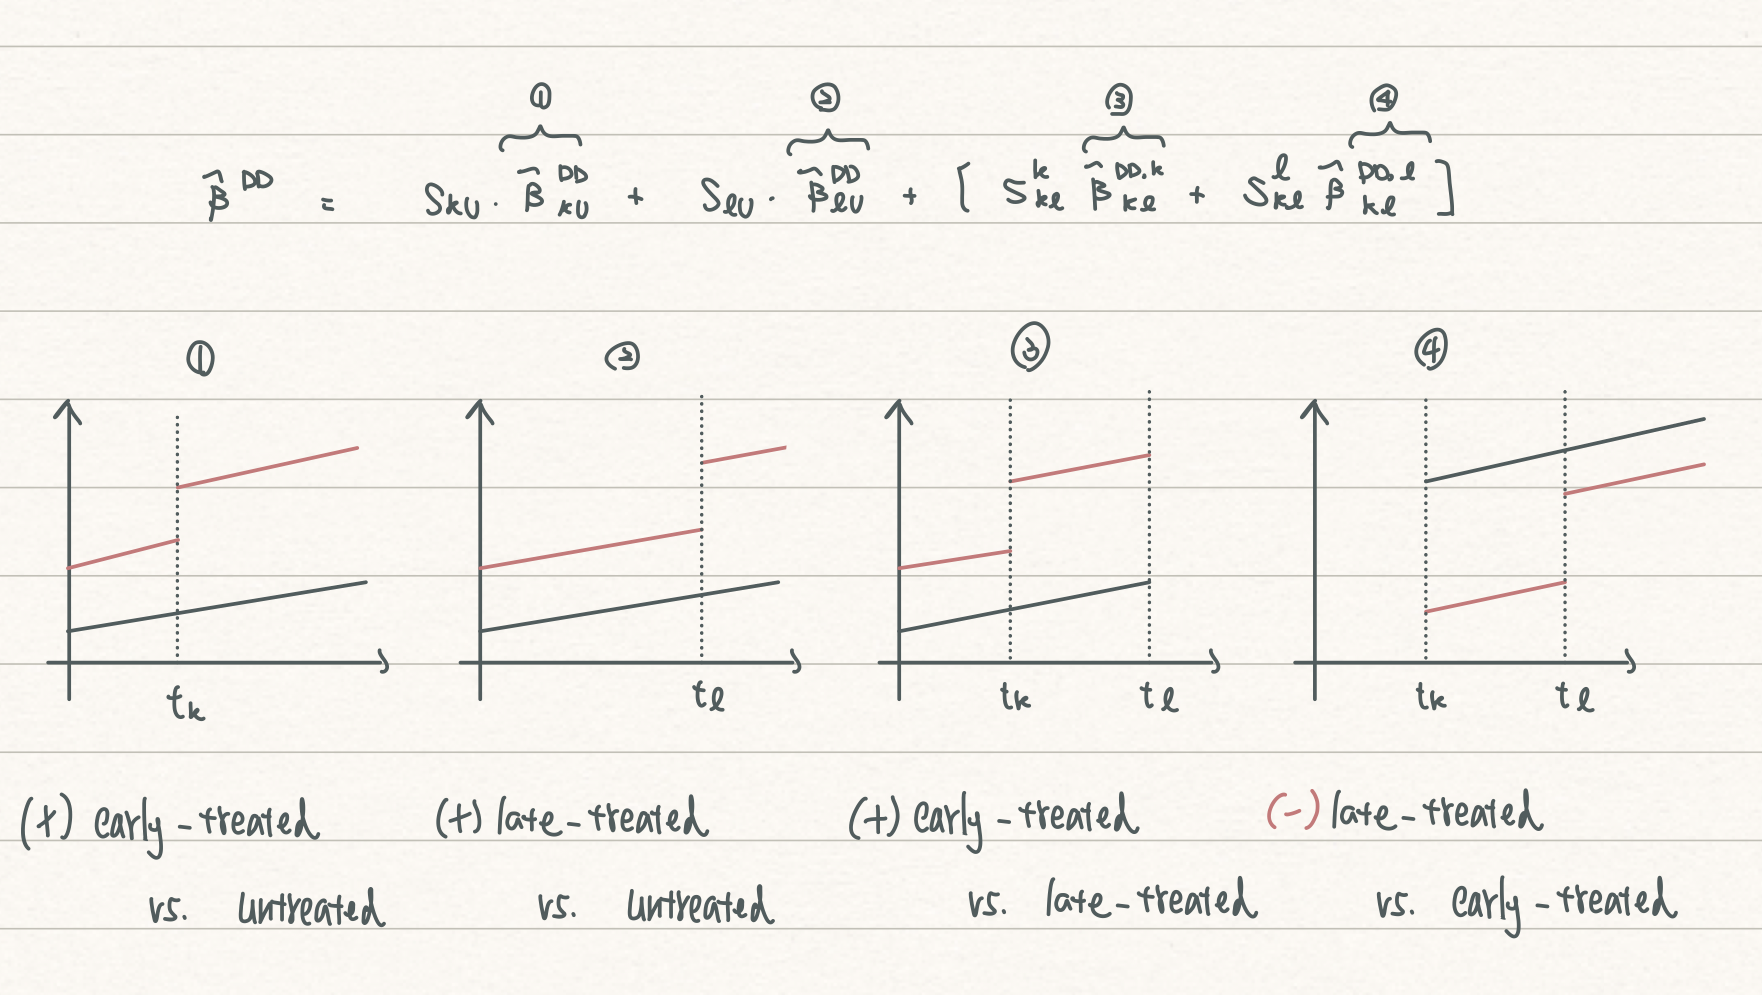
\includegraphics[scale = 0.2]{Q5a_TWFE.png}
            \end{solution}

        \item Simulate a data to illustrate your point above.
        
            \begin{solution}
                Follow the procedure of Pedro H. C. Sant'Anna and Brantly Callaway (2021), we use the code below to build data:
                \begin{lstlisting}[language=R]
    # Load required libraries
    library(tidyverse)
    library(lfe)
    library(fastDummies)
    library(ggthemes)
    library(did)
    theme_set(theme_clean() + theme(plot.background = element_blank()))

    # random seed
    iseed  = 20201221
    nrep <- 100  
    true_mu <- 1
    set.seed(iseed)

    # Data generating process
    make_data <- function(nobs = 1000, nstates = 40) {
  
    # unit fixed effects (unobserved heterogeneity)
    unit <- tibble(
        unit = 1:nobs,
        state = sample(1:nstates, nobs, replace = TRUE),
        unit_fe = rnorm(nobs, state/5, 1),
        mu = true_mu
    )
    
    # year fixed effects (first part)
    year <- tibble(
        year = 1980:2010,
        year_fe = rnorm(length(year), 0, 1)
    )
    
    # Put the states into treatment groups
    treat_taus <- tibble(
        state = sample(1:nstates, nstates, replace = FALSE),
        cohort_year = sort(rep(c(1986, 1992, 1998, 2004), 10))
    )
    
    expand_grid(unit = 1:nobs, year = 1980:2010) %>% 
        left_join(., unit) %>% 
        left_join(., year) %>% 
        left_join(., treat_taus) %>% 
        mutate(error = rnorm(nobs*31, 0, 1),
            treat = ifelse(year >= cohort_year, 1, 0),
            tau = ifelse(treat == 1, mu, 0),
            year_fe = year_fe + 0.1*(year - cohort_year)
        ) %>% 
        group_by(unit) %>% 
        mutate(tau_cum = cumsum(tau)) %>% 
        ungroup() %>% 
        mutate(dep_var = (2010 - cohort_year) + unit_fe + year_fe + tau_cum + error)
    }

    # Generate the data
    data <- make_data()

    # Draw the graph
    plot1 <- data %>% 
    ggplot(aes(x = year, y = dep_var, group = unit)) + 
    geom_line(alpha = 1/8, color = "grey") + 
    geom_line(data = data %>% 
                group_by(cohort_year, year) %>% 
                summarize(dep_var = mean(dep_var)),
                aes(x = year, y = dep_var, group = factor(cohort_year),
                    color = factor(cohort_year)),
                size = 2) + 
    labs(x = "", y = "Value", color = "Treatment group   ") + 
    geom_vline(xintercept = 1986, color = '#E41A1C', size = 2) + 
    geom_vline(xintercept = 1992, color = '#377EB8', size = 2) + 
    geom_vline(xintercept = 1998, color = '#4DAF4A', size = 2) + 
    geom_vline(xintercept = 2004, color = '#984EA3', size = 2) + 
    scale_color_brewer(palette = 'Set1') + 
    theme(legend.position = 'bottom',
            axis.title = element_text(size = 14),
            axis.text = element_text(size = 12))  +
    ggtitle("One draw of the DGP with homogeneous effects across cohorts \n and with all groups being eventually treated") +
    theme(plot.title = element_text(hjust = 0.5, size = 12))

    # plot
    plot1
                \end{lstlisting}

            and the data looks like
            \begin{center}
                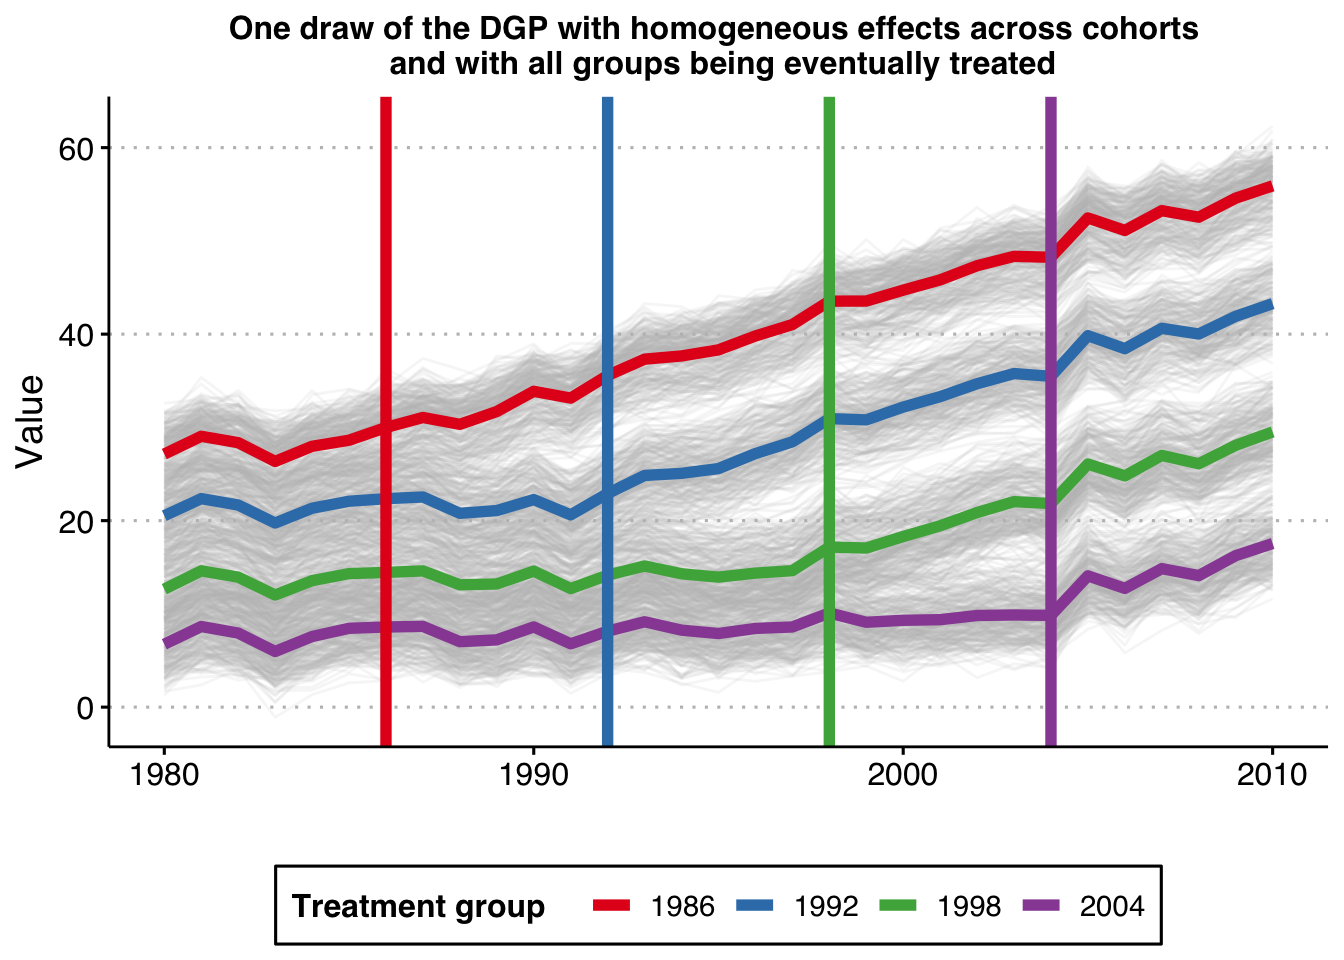
\includegraphics[scale = 0.3]{Q5b_TWFE.png}
            \end{center}

            Next, we utilize two-way fixed effect model to estimate

            \begin{lstlisting}
    # variables we will use
    keepvars <- c("`rel_year_-5`",  "`rel_year_-4`",  "`rel_year_-3`",  "`rel_year_-2`",
                "rel_year_0", "rel_year_1", "rel_year_2", "rel_year_3", "rel_year_4", "rel_year_5")

    run_ES_DiD <- function(...) {
    
    # resimulate the data
    data <- make_data()
    
    # make dummy columns
    data <- data %>% 
        # make dummies
        mutate(rel_year = year - cohort_year) %>% 
        dummy_cols(select_columns = "rel_year") %>% 
        # generate pre and post dummies
        mutate(Pre = ifelse(rel_year < -5, 1, 0),
            Post = ifelse(rel_year > 5, 1, 0))
    
    # estimate the model
    mod <- lfe::felm(dep_var ~ Pre + `rel_year_-5` + `rel_year_-4` + `rel_year_-3` + `rel_year_-2` + 
                    `rel_year_0` + `rel_year_1` + `rel_year_2` + `rel_year_3` + `rel_year_4` + 
                    `rel_year_5` + Post | unit + year | 0 | state, data = data, exactDOF = TRUE)
    
    # grab the obs we need
    mod2 <- tibble(
        estimate = mod$coefficients,
        term1 = rownames(mod$coefficients)
        )
    
    es <-
    mod2 %>% 
        filter(term1 %in% keepvars) %>% 
        mutate(t = c(-5:-2, 0:5)) %>% 
        select(t, estimate)
    es
    }

    # Run ES DID multiple times
    data_classical <- map_dfr(1:nrep, run_ES_DiD)

    # Draw the graph
    colors <- c("True Effect" = "red", "Estimated Effect" = "blue")

    ES_plot_classical <- data_classical %>% 
    group_by(t) %>% 
    summarize(avg = mean(estimate),
                sd = sd(estimate),
                lower.ci = avg - 1.96*sd,
                upper.ci = avg + 1.96*sd) %>% 
    bind_rows(tibble(t = -1, avg = 0, sd = 0, lower.ci = 0, upper.ci = 0)) %>% 
    mutate(true_tau = ifelse(t >= 0, (t + 1)* true_mu, 0)) %>% 
    ggplot(aes(x = t, y = avg)) + 
    geom_ribbon(aes(ymin = lower.ci, ymax = upper.ci), color = "lightgrey", alpha = 0.2) +
    geom_point(color = 'blue', size = 3) + 
    geom_line(aes(color = 'Estimated Effect'), size = 1) + 
    geom_line(aes(x = t, y = true_tau, color = 'True Effect'), linetype = "dashed", size = 2) + 
    geom_hline(yintercept = 0, linetype = "dashed") + 
    scale_x_continuous(breaks = -5:5) + 
    labs(x = "Relative Time", y = "Estimate") + 
    theme(axis.title = element_text(size = 14),
            axis.text = element_text(size = 12)) +
    ggtitle("TWFE event-study regression with binned end-points")+
    scale_color_manual(values = colors) + 
    theme(plot.title = element_text(hjust = 0.5, size = 12),
            legend.position = "bottom", 
            legend.title = element_blank())

    ES_plot_classical
            \end{lstlisting}

            where the estimation result is Biased.

            \begin{center}
                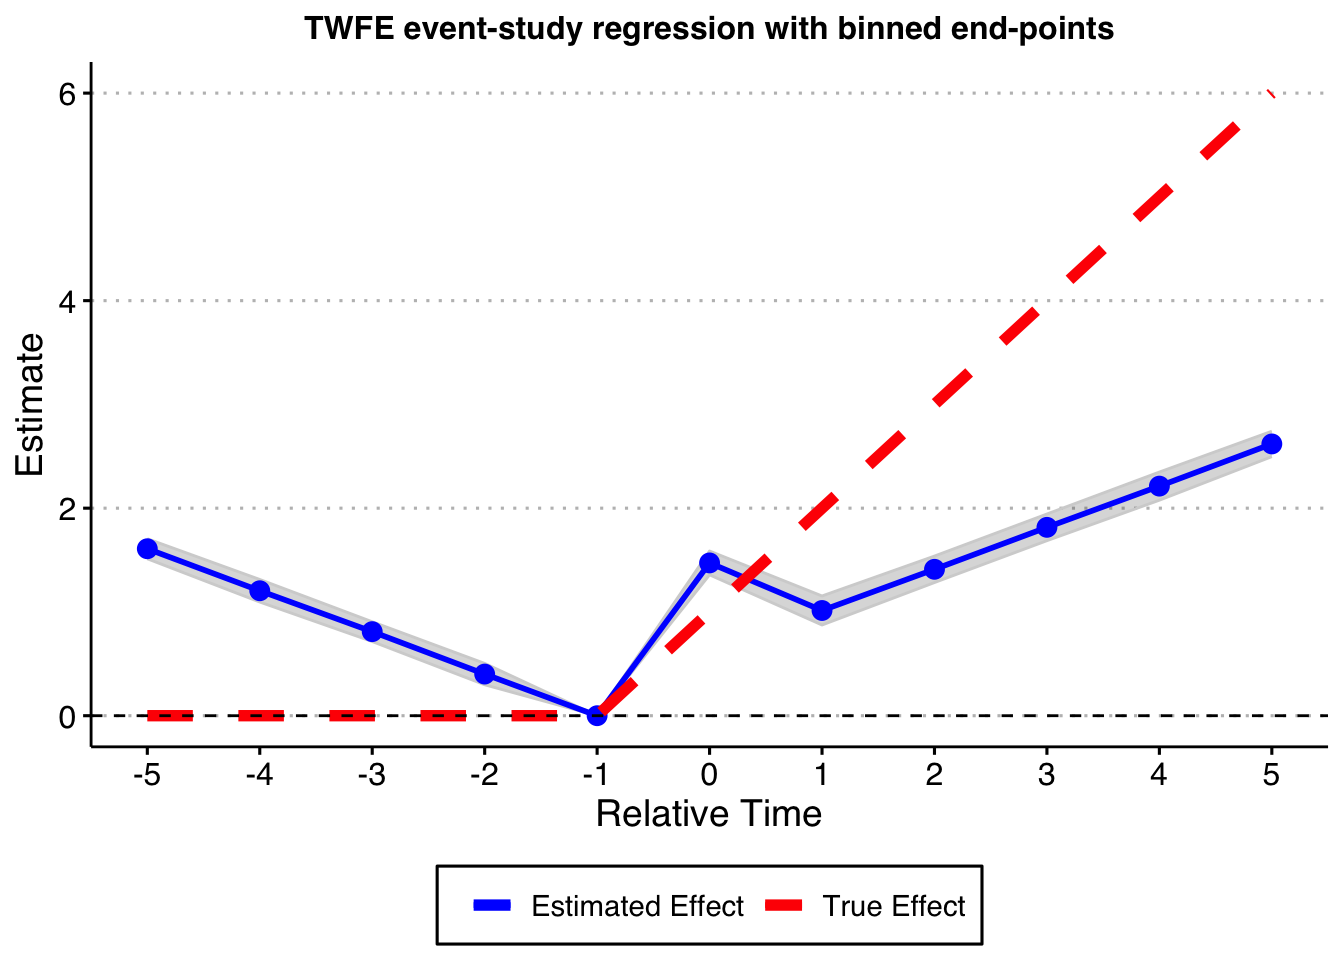
\includegraphics[scale = 0.3]{Q5b_TWFE_2.png}
            \end{center}

            \end{solution}    

        \item Look up the paper ``What's Trending in Difference-in-Differences? A Synthesis of the Recent Econometrics Literature.'' Learn to use one of the packages listed in the paper's appendix. Show that you can recover one of the treatment effect from your simulation.
        
            \begin{solution}
                
                We use untreated group as control group and do the estimation again

                \begin{lstlisting}
    # function to run ES DID
    run_CS <- function(...) {

    # resimulate the data
    data <- make_data()

    mod <- did::att_gt(yname = "dep_var", 
                        tname = "year",
                        idname = "unit",
                        gname = "cohort_year",
                        control_group= "notyettreated",
                        bstrap = FALSE,
                        data = data,
                        print_details = FALSE)
    event_std <- did::aggte(mod, type = "dynamic")

    att.egt <- event_std$att.egt
    names(att.egt) <- event_std$egt

    # grab the obs we need
    broom::tidy(att.egt) %>% 
        filter(names %in% -5:5) %>% 
        mutate(t = -5:5, estimate = x) %>% 
        select(t, estimate)
    }

    data_CS <- map_dfr(1:nrep, run_CS)

    ES_plot_CS <- data_CS %>% 
    group_by(t) %>% 
    summarize(avg = mean(estimate),
                sd = sd(estimate),
                lower.ci = avg - 1.96*sd,
                upper.ci = avg + 1.96*sd) %>% 
    mutate(true_tau = ifelse(t >= 0, (t + 1)* true_mu, 0)) %>% 
    ggplot(aes(x = t, y = avg)) + 
    #geom_linerange(aes(ymin = lower.ci, ymax = upper.ci), color = 'darkgrey', size = 2) + 
    geom_ribbon(aes(ymin = lower.ci, ymax = upper.ci), color = "lightgrey", alpha = 0.2) +
    geom_point(color = 'blue', size = 3) + 
    geom_line(aes(color = 'Estimated Effect'), size = 1) + 
    geom_line(aes(x = t, y = true_tau, color = 'True Effect'), linetype = "dashed", size = 2) + 
    geom_hline(yintercept = 0, linetype = "dashed") + 
    scale_x_continuous(breaks = -5:5) + 
    labs(x = "Relative Time", y = "Estimate") + 
    theme(axis.title = element_text(size = 14),
            axis.text = element_text(size = 12)) +
    ggtitle("Event-study-parameters estimated using Callaway and Sant'Anna (2020)\nComparison group: Not-yet-treated")+
        scale_color_manual(values = colors) + 
    theme(plot.title = element_text(hjust = 0.5, size=12),
            legend.position = "bottom", 
            legend.title = element_blank())

    ES_plot_CS
                \end{lstlisting}

            which gives us the correct estimation of treatment effect

            \begin{center}
                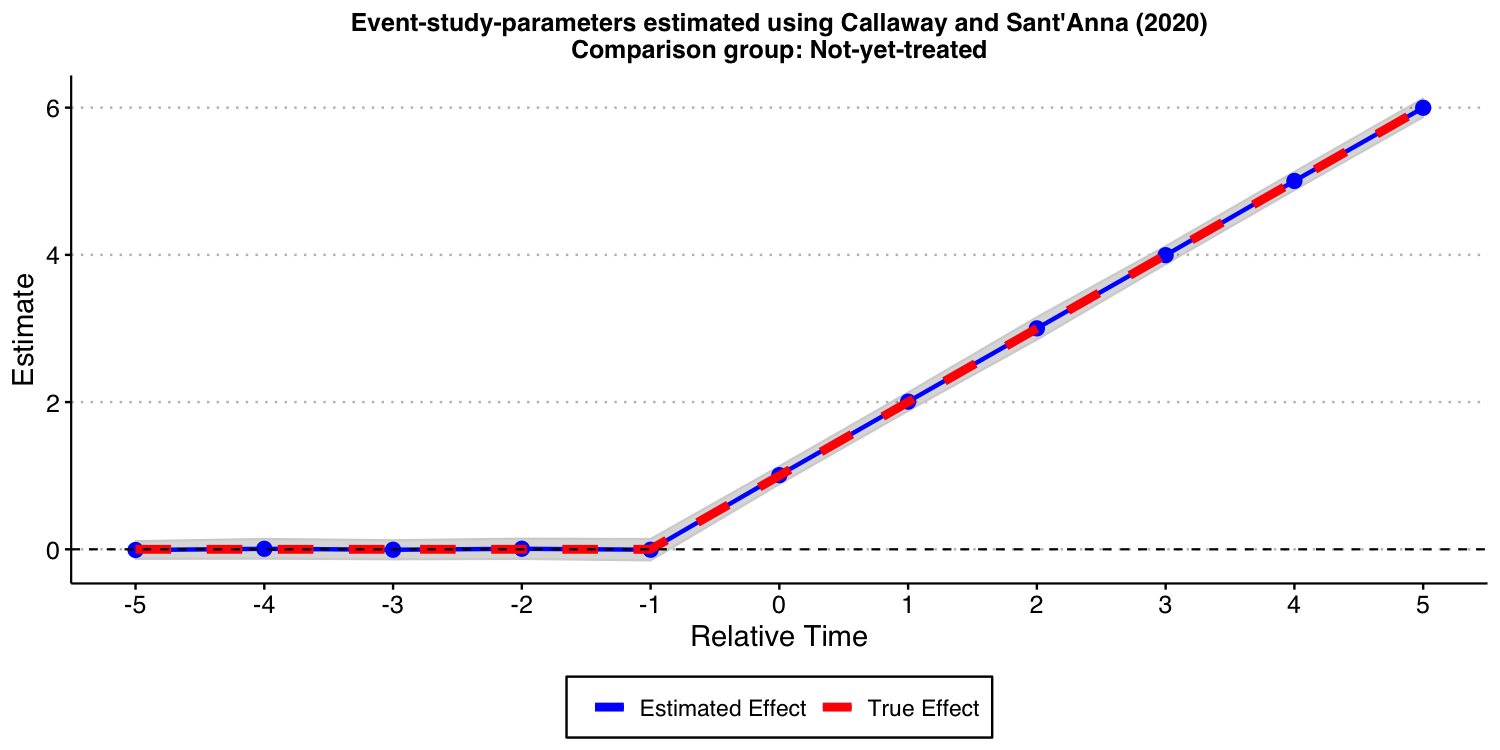
\includegraphics[scale = 0.25]{Q5c_TWFE.png}
            \end{center}

            \end{solution}

    \end{enumerate}




\end{document}  